\documentclass[10pt]{beamer}

\usetheme[progressbar=frametitle]{metropolis}
\usepackage{appendixnumberbeamer}
\usepackage{textgreek}
\usepackage{booktabs}
\usepackage[scale=2]{ccicons}
\usepackage{fontawesome}
\usepackage{pgfplots}
\usepgfplotslibrary{dateplot}
\usepackage{mathtools}
\usepackage{xspace}
\usepackage{wrapfig}
\newcommand{\themename}{\textbf{\textsc{metropolis}}\xspace}
%\usepackage{caption}
%\usepackage{hyperref}
%\usepackage[citestyle=authoryear,natbib=true,backend=bibtex]{biblatex}
%\usepackage{biblatex}
%\bibliography{rl}
%\usepackage{natbib}

\title{A Brief Survey of Reinforcement Learning}
\subtitle{A modern beamer theme}
\date{\today}
% \date{11 Dec 2018}
\author{Giancarlo Frison}
%\institute{ \faTwitter gfrison}
% \titlegraphic{\hfill\includegraphics[height=1.5cm]{logo.pdf}}
\begin{document}

\setbeamertemplate{frame footer}{\faTwitter gfrison 2018}

\maketitle

\begin{frame}{Table of contents}
  \setbeamertemplate{section in toc}[sections numbered]
  \tableofcontents[hideallsubsections]
\end{frame}

\section{Introduction}
\begin{frame}[fragile]{What is Reinforcement Learning}
	\begin{figure}[t!]	
	\centering
	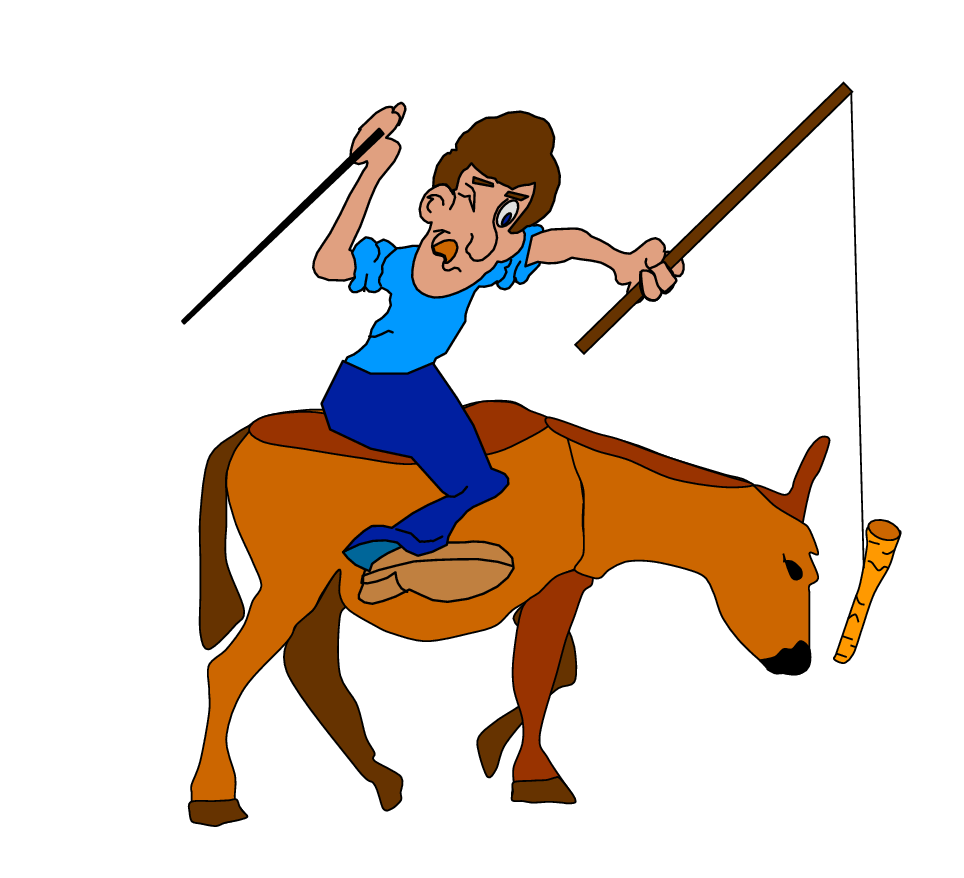
\includegraphics[scale=0.3]{img/donkey.png}
	\cite{donkey}
	\end{figure}
	\textsc{Reinforcement learning} is an area of machine learning concerned with how software agents ought to take actions in an environment so as to maximize some notion of cumulative reward.
\end{frame}

\begin{frame}[fragile]{Challenges in RL}
	RL  vision  is about creating  systems that  are  capable  of  learning  how  to  adapt  in  the  real  world, solely based on trial-and-error.
	
	Challenges:
	\begin{itemize}
		\item The  optimal  policy  must  be  inferred  by  interacting with the environment. The only learning signal
the agent receives is the reward.
		\item Agents  must  deal  with  long-range  time  dependencies:
Often the consequences of an action only materialise after
many transitions of the environment \cite{Montague1999}.
	\end{itemize}
\end{frame}

\begin{frame}[fragile]{What it is Not}
Although RL can induce to an optimization, there are major differences within:
  \begin{itemize}[<+- | alert@+>]
    \item {Supervised learning}
	\item Mathematical optimization
	\item Genetic programming
  \end{itemize}
\end{frame}

\section{Genetic Programming}
\begin{frame}{Genetic Programming}
	\textsc{GP} is a technique whereby computer programs are encoded as a set of genes that are then modified using an evolutionary algorithm.
	\begin{itemize}
		\item A number of chromosomes are randomly created.
		\item Each chromosome is evaluated through a fitness function.
		\item Best ones are selected, the others are disposed.
		\item Chromosomes could be breded among the selected for a new generation.
		\item Offsprings are randomly mutated.
		\item Repeat until the score threshold is reached \cite{gf-gp}.
	\end{itemize}
\end{frame}

\begin{frame}{Crossover}
	\begin{figure}
		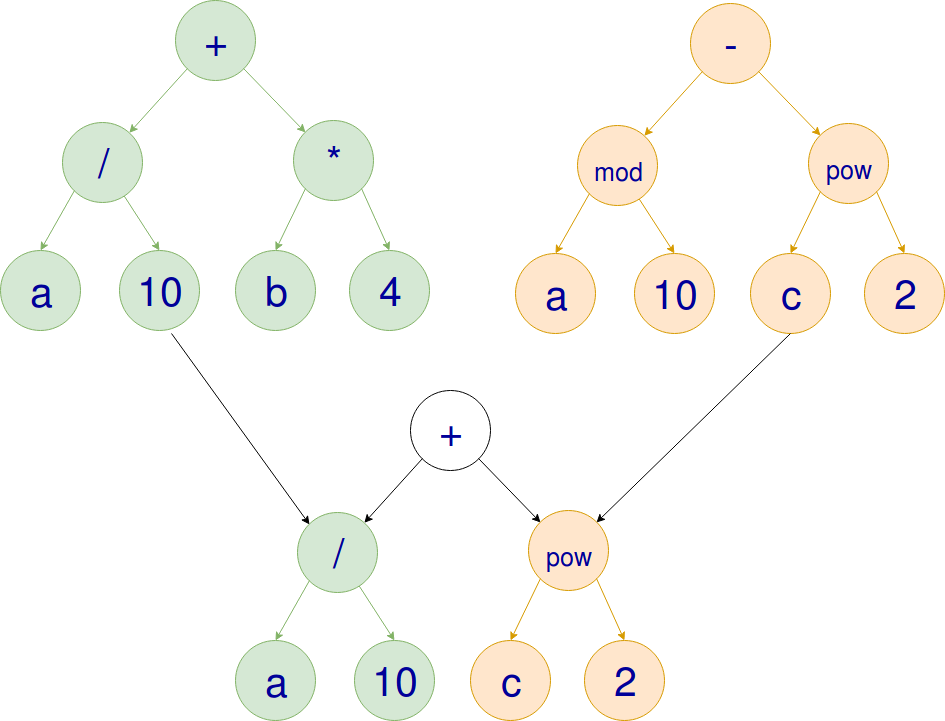
\includegraphics[scale=0.15]{img/ast-crossover.png}
		\caption{The “breeding” is called crossover. The chromosome (in this case an \textsc{AST}), is merged between two individuals for searching a better function.}
	\end{figure}	
\end{frame}

\begin{frame}{Strenghts on many local minima}
\textsc{GP} may overtake gradient-based algorithms when the solution space has many local minima
	\begin{figure}
		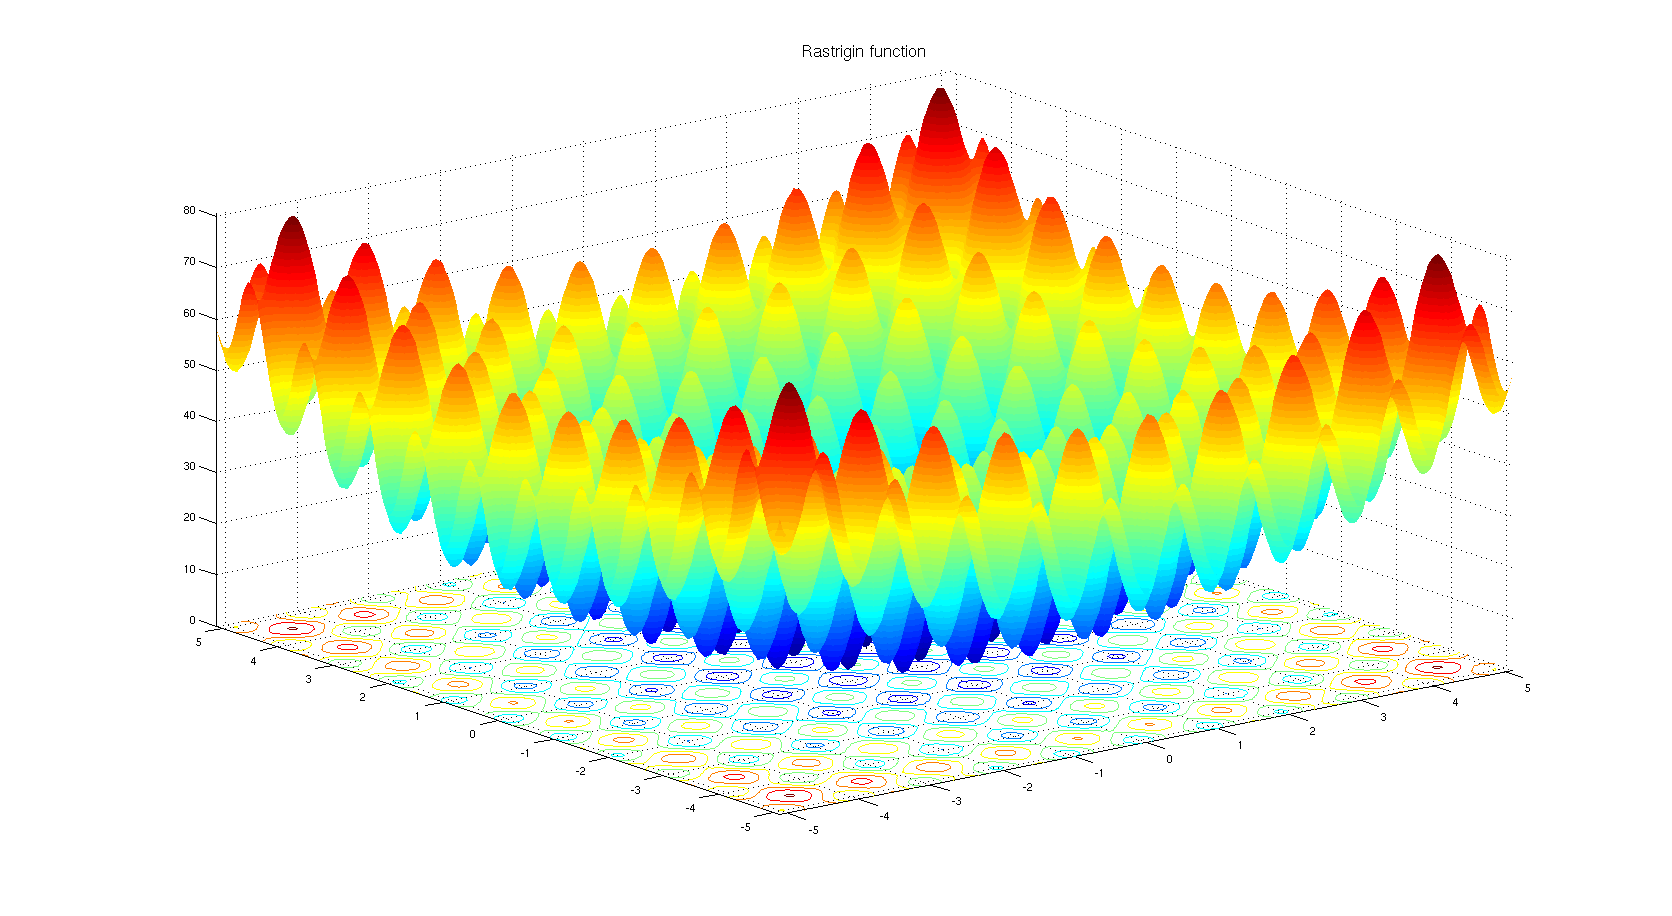
\includegraphics[scale=0.16]{img/Rastrigin_function.png}
		\caption{Rastrigin function}
	\end{figure}
\end{frame}

\begin{frame}{Strenghts on no-differentiable functions}
$f(x)$ is \textsc{differentiable} when it has always a finite derivative along the domain. 
	\begin{figure}
		\begin{tikzpicture}[scale=0.5]
			\begin{axis}[
			    xmin=-2, xmax=2,
			    ymin=-1, ymax=2,
			    axis lines=center,
			    axis on top=true,
			    domain=-1:1,
			    ]
			
			    \addplot [mark=none,draw=red,ultra thick] {abs(x)};
			\end{axis}
		\end{tikzpicture}
	    \caption{$f(x) = |x|$ has no derivative at $x = 0$.}
	\end{figure}
\textsc{GP} is tollerant to \emph{latent} no-differentiable functions.	
\end{frame}

\section{Multi-armed Bandit}
\begin{frame}{Multi-armed Bandit}
	\begin{figure}[t!]	
	\centering
	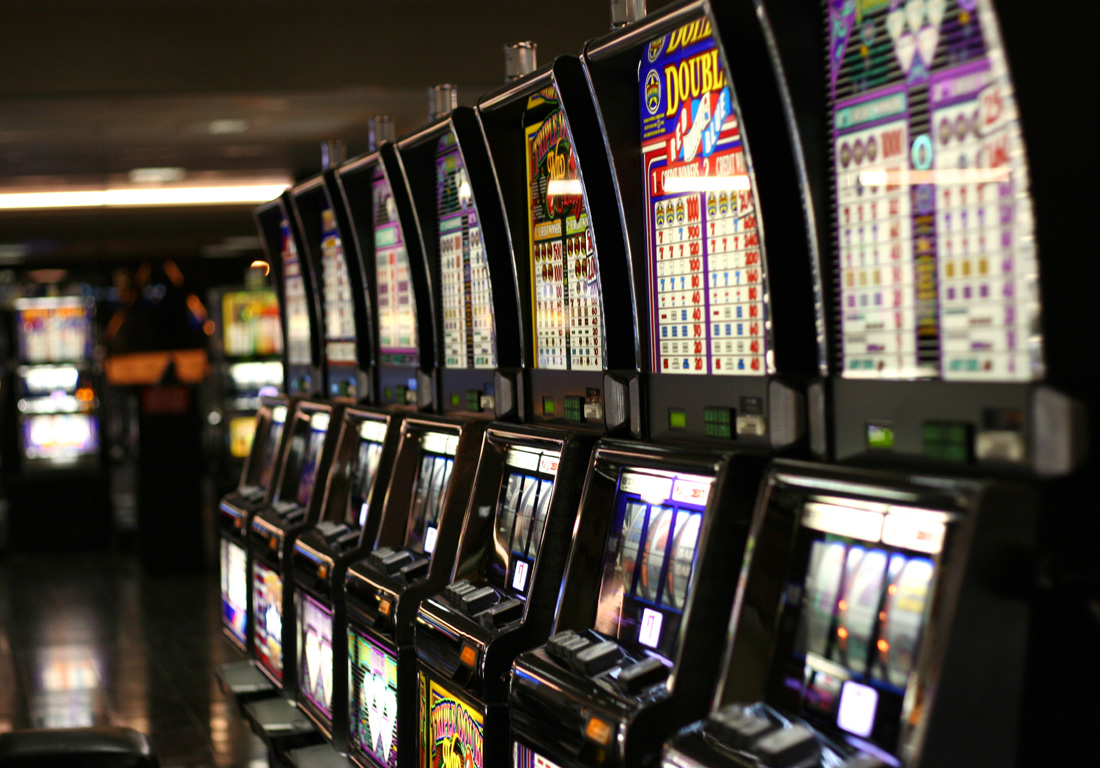
\includegraphics[scale=0.2]{img/Las_Vegas_slot_machines.jpg}
	\end{figure}
	The multi-armed bandit problem has been the subject of decades of intense study in statistics, operations research, electrical engineering, computer science, and economics \cite{bandit}
\end{frame}

\begin{frame}
	\frametitle{\begin{math} Q \end{math} Value's Action}
	\begin{figure}[t!]
		\centering
		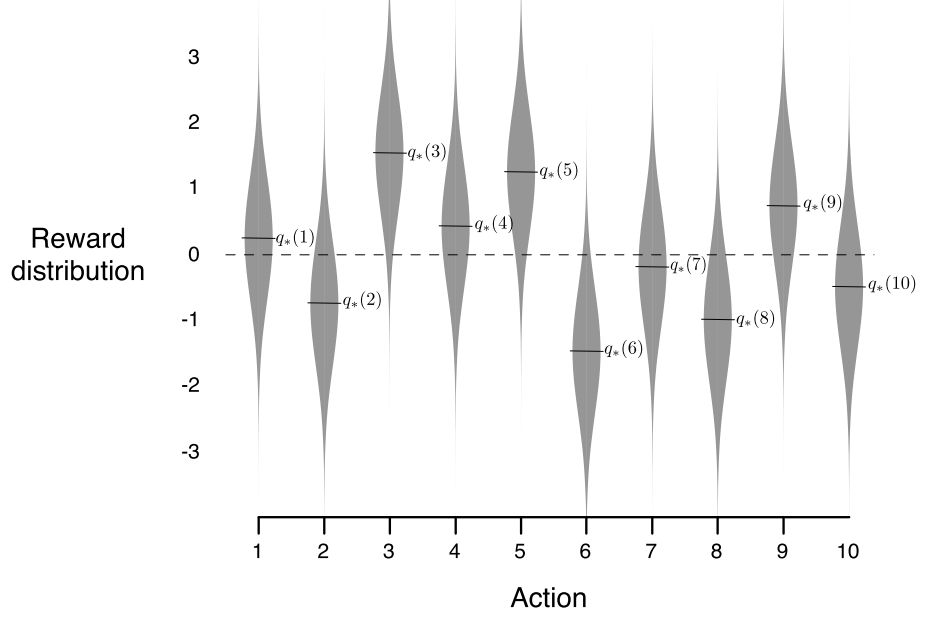
\includegraphics[scale=0.25]{img/bandit-reward-dist.png}
	\end{figure}
	An example bandit problem \cite{Montague1999}. Obtained measures after repeated pullings with 10 arms.
\end{frame}

\begin{frame}
	\frametitle{\begin{math} Q \end{math} Value's Action}
	\begin{math} \mathbf{Q_n} \end{math} is the estimated value of its action after $ n $ selections.	
	$$ Q_{n+1} = \frac{R_1 +R_2 + ... +R_{n}}{n} $$
	A more scalable formula, updates the average with incremental and small constant:
	$$ Q_{n+1} = Q_n + \frac{1}{n}(R_n-Q_n)$$
	General expression of the badint algorithm at the fundation of RL. \begin{math}Target\end{math} could be considered the reward $ R $ by now.
	$$ \mathbf{NewEstimate = OldEstimate + StepSize(Target-OldEstimate)}$$
\end{frame}

\begin{frame}
\frametitle{Gambler's Dilemma}
When pulled, an arm produces a random payout drawn independently of the past. Because the distribution of payouts corresponding to each arm is not listed, the player can learn it only by experimenting.
	\begin{columns}
		\begin{column}{0.5\textwidth}
			\begin{alertblock}{Exploitation}
		Earn more money by exploiting arms that yielded high payouts in the past.
			\end{alertblock}
		\end{column}
		\begin{column}{0.5\textwidth}  %%<--- here
			\begin{alertblock}{Exploration}
		Exploring alternative arms may return higher payouts in the future.
			\end{alertblock}
		\end{column}
	\end{columns}
\end{frame}

\section{Markov Decision Process}
\begin{frame}
	\frametitle{Definition of MDP}
	\begin{figure}
		\includegraphics[scale=0.15]{img/2015_DARPA_Robotics_Challenge_150606-N-PO203-090.jpg}	
		\caption{2015 DARPA Robotics Challange \cite{mdp-robot}}
	\end{figure}
	Despite as in bandits, MDP formalizes the decision making (Policy $\pi$) in sequential steps, aggregated in Episodes. 
\end{frame}

\begin{frame}
	\frametitle{Actions and States}
	\begin{figure}
	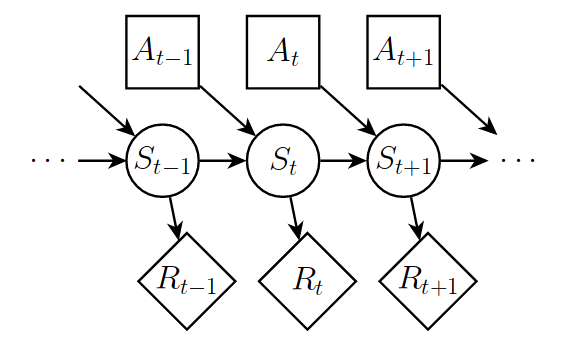
\includegraphics[scale=0.2]{img/mdp-states.png}
	\caption{Model representation of MDP \cite{mdp-process}}
	\end{figure}
	MDP strives to find the best $\pi$ to all possible states. 
	In Markov processes, the selected action depends \textbf{only} on current state.
\end{frame}

\begin{frame}
	\frametitle{How to evaluate an Agent?}
	Given that:
	\begin{itemize}
		\item Policy $\pmb{\pi}$ defines a particular way of acting.
		\item $\mathbf{v_π(s)}$ is the expected return from $\mathbf{s}$ following $\pmb{\pi}$ \emph{thereafter}.
		\item $\mathbf{q_π(s, a)}$ is the $\mathbf{v_π(s)}$ taking action $\mathbf{a}$
		\item For maximizing future rewards, only the $\mathbf{max}$ $Q_\pi$ is considered. 
		\item $\pmb{\gamma}$ is the rewards' discount factor. 
	\end{itemize}
	
	A recursive algorithm could be indentified, known as the \textsc{Bellman equation}. Iteratevely computes the value $\mathbf{Q}$ from the terminal state:
	$$ \mathbf{Q_t(s, a) = R_{t + 1} + \gamma max[v(S_{t+1})]} $$

	
		
\end{frame}

\begin{frame}
	\frametitle{Grid World}
	\begin{columns}
		\begin{column}{0.5\textwidth}
			\begin{tikzpicture}[scale=2]
			\draw[step=0.5cm,color=gray] (-1,-1) grid (1,1);
			\node at (-0.75,+0.75) { \faFlagCheckered };
			\node at (-0.25,+0.75) {-1};
			\node at (+0.25,+0.75) {-1};
			\node at (+0.75,+0.75) {-1};
			\node at (-0.75,+0.25) {-1};
			\node at (-0.25,+0.25) {-1};
			\node at (+0.25,+0.25) {-1};
			\node at (+0.75,+0.25) {-1};
			\node at (-0.75,-0.25) {-1};
			\node at (-0.25,-0.25) {-1};
			\node at (+0.25,-0.25) {-1};
			\node at (+0.75,-0.25) {-1};

			\node at (-0.75,-0.75) {-1};
			\node at (-0.25,-0.75) {-1};
			\node at (+0.25,-0.75) {-1};
			\node at (+0.75,-0.75) { \faFlagCheckered  };
			\end{tikzpicture}
		\end{column}
		\begin{column}{0.5\textwidth} 
			\begin{itemize}
				\item $ A = {up, down, right, left}$
				\item Terminal states are the flagged boxes.		
				\item $R_t = 0$ for terminal states.
				\item $R_t = -1$ for other states.
			\end{itemize}			 
		\end{column}
	\end{columns}
	The problem is to define the best $\pmb{\pi}$. Value function is computed by iterative policy evaluation. 
\end{frame}
\begin{frame}{Iteration 1}
	\begin{columns}
		\begin{column}{0.1\textwidth}
		\end{column}
		\begin{column}{0.4\textwidth}
			\textbf{Calculated $V_1$}
		\end{column}
		\begin{column}{0.4\textwidth} 
			\textbf{Policy $\pi_1$}
		\end{column}
		\begin{column}{0.1\textwidth}
		\end{column}
	\end{columns}
	\begin{columns}
		\begin{column}{0.1\textwidth}
		\end{column}
		\begin{column}{0.4\textwidth}
			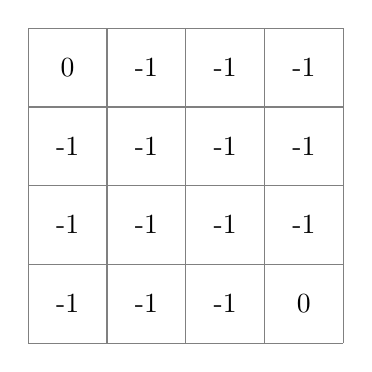
\begin{tikzpicture}[scale=2]
			\draw[step=0.5cm,color=gray] (-1,-1) grid (1,1);
			\node at (-0.75,+0.75) { 0 };
			\node at (-0.25,+0.75) {-1};
			\node at (+0.25,+0.75) {-1};
			\node at (+0.75,+0.75) {-1};
			\node at (-0.75,+0.25) {-1};
			\node at (-0.25,+0.25) {-1};
			\node at (+0.25,+0.25) {-1};
			\node at (+0.75,+0.25) {-1};
			\node at (-0.75,-0.25) {-1};
			\node at (-0.25,-0.25) {-1};
			\node at (+0.25,-0.25) {-1};
			\node at (+0.75,-0.25) {-1};

			\node at (-0.75,-0.75) {-1};
			\node at (-0.25,-0.75) {-1};
			\node at (+0.25,-0.75) {-1};
			\node at (+0.75,-0.75) { 0  };
			\end{tikzpicture}
		\end{column}
		\begin{column}{0.4\textwidth} 
			\begin{tikzpicture}[scale=2]
			\draw[step=0.5cm,color=gray] (-1,-1) grid (1,1);
			\node at (-0.75,+0.75) { \faFlagCheckered };
			\node at (-0.25,+0.75) { $\leftarrow$ };
			\node at (+0.25,+0.75) {?};
			\node at (+0.75,+0.75) {?};
			\node at (-0.75,+0.25) {$\uparrow$};
			\node at (-0.25,+0.25) {?};
			\node at (+0.25,+0.25) {?};
			\node at (+0.75,+0.25) {?};
			\node at (-0.75,-0.25) {?};
			\node at (-0.25,-0.25) {?};
			\node at (+0.25,-0.25) {?};
			\node at (+0.75,-0.25) {$\downarrow$};

			\node at (-0.75,-0.75) {?};
			\node at (-0.25,-0.75) {?};
			\node at (+0.25,-0.75) {$\rightarrow$};
			\node at (+0.75,-0.75) { \faFlagCheckered  };
			\end{tikzpicture}
		\end{column}
		\begin{column}{0.1\textwidth}
		\end{column}
	\end{columns}

\end{frame}
\begin{frame}{Iteration 2}
	\begin{columns}
		\begin{column}{0.1\textwidth}
		\end{column}
		\begin{column}{0.4\textwidth}
			\textbf{Calculated $V_2$}
		\end{column}
		\begin{column}{0.4\textwidth} 
			\textbf{Policy $\pi_2$}
		\end{column}
		\begin{column}{0.1\textwidth}
		\end{column}
	\end{columns}
	\begin{columns}
		\begin{column}{0.1\textwidth}
		\end{column}
		\begin{column}{0.4\textwidth}
			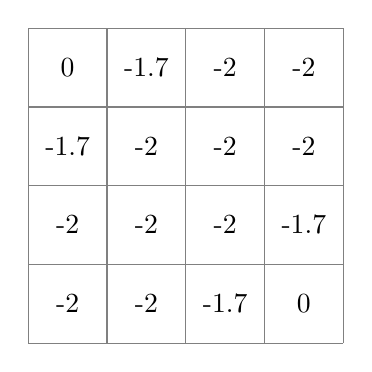
\begin{tikzpicture}[scale=2]
			\draw[step=0.5cm,color=gray] (-1,-1) grid (1,1);
			\node at (-0.75,+0.75) { 0 };
			\node at (-0.25,+0.75) {-1.7};
			\node at (+0.25,+0.75) {-2};
			\node at (+0.75,+0.75) {-2};
			\node at (-0.75,+0.25) {-1.7};
			\node at (-0.25,+0.25) {-2};
			\node at (+0.25,+0.25) {-2};
			\node at (+0.75,+0.25) {-2};
			\node at (-0.75,-0.25) {-2};
			\node at (-0.25,-0.25) {-2};
			\node at (+0.25,-0.25) {-2};
			\node at (+0.75,-0.25) {-1.7};

			\node at (-0.75,-0.75) {-2};
			\node at (-0.25,-0.75) {-2};
			\node at (+0.25,-0.75) {-1.7};
			\node at (+0.75,-0.75) { 0  };
			\end{tikzpicture}
		\end{column}
		\begin{column}{0.4\textwidth} 
			\begin{tikzpicture}[scale=2]
			\draw[step=0.5cm,color=gray] (-1,-1) grid (1,1);
			\node at (-0.75,+0.75) { \faFlagCheckered };
			\node at (-0.25,+0.75) { $\leftarrow$ };
			\node at (+0.25,+0.75) { $\leftarrow$ };
			\node at (+0.75,+0.75) {?};
			\node at (-0.75,+0.25) {$\uparrow$};
			\node at (-0.25,+0.25) {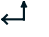
\includegraphics[scale=0.25]{img/left-up.png}	};
			\node at (+0.25,+0.25) {?};
			\node at (+0.75,+0.25) {$\downarrow$};
			\node at (-0.75,-0.25) { $\uparrow$ };
			\node at (-0.25,-0.25) {?};
			\node at (+0.25,-0.25) {
\includegraphics[scale=0.25]{img/down-right.png}};
			\node at (+0.75,-0.25) {$\downarrow$};

			\node at (-0.75,-0.75) {?};
			\node at (-0.25,-0.75) {$\rightarrow$};
			\node at (+0.25,-0.75) {$\rightarrow$};
			\node at (+0.75,-0.75) { \faFlagCheckered  };
			\end{tikzpicture}
		\end{column}
		\begin{column}{0.1\textwidth}
		\end{column}
	\end{columns}

\end{frame}
\begin{frame}{Iteration 3}
	\begin{columns}
		\begin{column}{0.1\textwidth}
		\end{column}
		\begin{column}{0.4\textwidth}
			\textbf{Calculated $V_3$}
		\end{column}
		\begin{column}{0.4\textwidth} 
			\textbf{Policy $\pi_3$}
		\end{column}
		\begin{column}{0.1\textwidth}
		\end{column}
	\end{columns}
	\begin{columns}
		\begin{column}{0.1\textwidth}
		\end{column}
		\begin{column}{0.4\textwidth}
			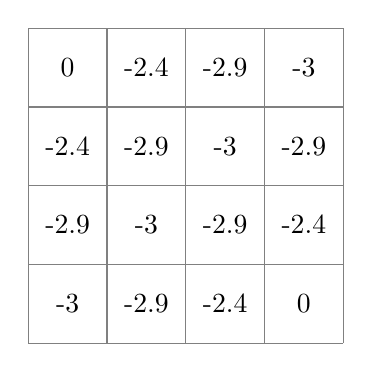
\begin{tikzpicture}[scale=2]
			\draw[step=0.5cm,color=gray] (-1,-1) grid (1,1);
			\node at (-0.75,+0.75) { 0 };
			\node at (-0.25,+0.75) {-2.4};
			\node at (+0.25,+0.75) {-2.9};
			\node at (+0.75,+0.75) {-3};
			\node at (-0.75,+0.25) {-2.4};
			\node at (-0.25,+0.25) {-2.9};
			\node at (+0.25,+0.25) {-3};
			\node at (+0.75,+0.25) {-2.9};
			\node at (-0.75,-0.25) {-2.9};
			\node at (-0.25,-0.25) {-3};
			\node at (+0.25,-0.25) {-2.9};
			\node at (+0.75,-0.25) {-2.4};

			\node at (-0.75,-0.75) {-3};
			\node at (-0.25,-0.75) {-2.9};
			\node at (+0.25,-0.75) {-2.4};
			\node at (+0.75,-0.75) { 0  };
			\end{tikzpicture}
		\end{column}
		\begin{column}{0.4\textwidth} 
			\begin{tikzpicture}[scale=2]
			\draw[step=0.5cm,color=gray] (-1,-1) grid (1,1);
			\node at (-0.75,+0.75) { \faFlagCheckered };
			\node at (-0.25,+0.75) { $\leftarrow$ };
			\node at (+0.25,+0.75) { $\leftarrow$ };
			\node at (+0.75,+0.75) {
\includegraphics[scale=0.25]{img/down-left.png}};
			\node at (-0.75,+0.25) {$\uparrow$};
			\node at (-0.25,+0.25) {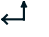
\includegraphics[scale=0.25]{img/left-up.png}	};
			\node at (+0.25,+0.25) {
\includegraphics[scale=0.25]{img/down-left.png}};
			\node at (+0.75,+0.25) {$\downarrow$};
			\node at (-0.75,-0.25) { $\uparrow$ };
			\node at (-0.25,-0.25) {
\includegraphics[scale=0.25]{img/down-right.png}};
			\node at (+0.25,-0.25) {
\includegraphics[scale=0.25]{img/down-right.png}};
			\node at (+0.75,-0.25) {$\downarrow$};

			\node at (-0.75,-0.75) {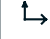
\includegraphics[scale=0.25]{img/up-right.png}};
			\node at (-0.25,-0.75) {$\rightarrow$};
			\node at (+0.25,-0.75) {$\rightarrow$};
			\node at (+0.75,-0.75) { \faFlagCheckered  };
			\end{tikzpicture}
		\end{column}
		\begin{column}{0.1\textwidth}
		\end{column}
	\end{columns}

\end{frame}

sc
\section{Neural Networks in RL}
\begin{frame}{Beyond the Gridworld}
	In the Gridworld every state value $\mathbf{v_t}$ is stored in a table. 
	The approach lacks scalability and is inherently limited to fairly low-dimension problems.
	\begin{figure}
		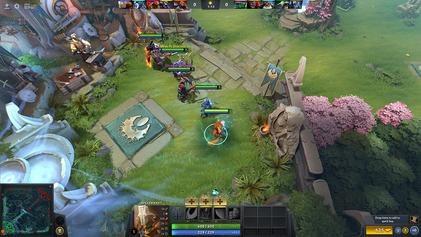
\includegraphics[scale=0.4]{img/dota2.jpg}
		\caption{The state $\mathbf{v_t}$ might be a frame of a videogame \cite{dota2}}
	\end{figure}
\end{frame}
\begin{frame}[fragile]{Deep Reinforcement Learning}
Deep  learning  enables  RL  to  scale  to  decision-making
problems  that  were  previously  intractable,  i.e.,  settings  with
high-dimensional  state  and  action  spaces. \cite{arulkumaran2017brief}
	\begin{itemize}
		\item \alert{Universal function approximator} Multilayer neural networks can approximate any continuous function to any degree of accuracy \cite{hornik1989multilayer}.
		\pause
		\item \alert{Representation learning} Automatically discover the representations needed for feature detection or classification from raw data, also known as \textsc{feature engeneering} \cite{bengio2013representation}.
	\end{itemize}
	Neural networks can learn the approximated value of $\mathbf{V_s}$ or $\mathbf{Q(s, a)}$ for any given \textsc{state/action space}.
\end{frame}

\begin{frame}{Discrete space}
	When the \textsc{action space} is limited by a set of options, \textit{(e.g. turn right, left)} the output layer could be a set of neurons as the number of possible actions.
	\begin{figure}
		\begin{tabular}{ |c|c|c|c| } 
		 \hline
			\textbf{A1} & \textbf{A2} & \textbf{A3} & \textbf{A4}  \\ [0.5ex] 
		 \hline
		 \hline
			 0.21 & 0.27 & \textbf{0.30} & 0.21 \\ 
		 \hline
		\end{tabular}
		\caption{Output layer with softmax}
	\end{figure}
	The choosed action is the one with the biggest $Q_t$ (\textsc{A3}).
\end{frame}

\begin{frame}{Exploration in discrete space}
	The balance between \textsc{exploration} and \textsc{exploitation} is one of the most challanging task in \textsc{RL}.
	The most common is the \textbf{\textepsilon-greedy}:
	\begin{equation}
  \pi(s)=\begin{cases}
    \text{random action}, & \text{if $\xi < \epsilon$}.\\
    argmax Q(s, a), & \text{otherwise}.
  \end{cases}
\end{equation}
	With \textsc{\textepsilon-greedy}, at each time step, the agent selects a random action with a fixed probability, $0 \leq \epsilon \leq 1$, instead of selecting the learned optimal action.
\end{frame}

\begin{frame}{Exploration in discrete space}
	\textsc{\textepsilon-greedy} must be tuned and it is fixed during the training. In contrast, \textsc{Value-Difference Based Exploration} adapts the exploration-probability based on fluctuations of confidence
	\cite{tokic2011value}.
	\begin{columns}
		\begin{column}{0.1\textwidth}\end{column}
		\begin{column}{0.4\textwidth}
	\begin{figure}
		\begin{tabular}{ |c|c|c|c| } 
		 \hline
			\textbf{A1} & \textbf{A2} & \textbf{A3} & \textbf{A4}  \\ [0.5ex] 
		 \hline
		 \hline
			 0.21 & 0.27 & \textbf{0.30} & 0.21 \\ 
		 \hline
		\end{tabular}
		\caption{Low confidence, flat likelihood}
	\end{figure}

		\end{column}
		\begin{column}{0.4\textwidth}
	\begin{figure}
		\begin{tabular}{ |c|c|c|c| } 
		 \hline
			\textbf{A1} & \textbf{A2} & \textbf{A3} & \textbf{A4}  \\ [0.5ex] 
		 \hline
		 \hline
			 0.21 & 0.07 & \textbf{0.70} & 0.01 \\ 
		 \hline
		\end{tabular}
		\caption{High confidence, sharp likelihood}
	\end{figure}

		\end{column}
		\begin{column}{0.1\textwidth}\end{column}
	\end{columns}
\end{frame}

\begin{frame}{Continuous space}
	Applications of \textsc{RL} require continuous state spaces defined by means of continuous variables \textit{e.g. position, velocity, torque}. 
	\begin{itemize}
		\item \begin{alertblock}{Single Output}		
				Like in \textsc{DDPG} algorithm. The \textsc{NN} yields only one output.
			\end{alertblock}
		\pause
		\item \begin{alertblock}{Probability distribution}
The network yields a distribution. For convenience usually it is a \textsc{normal distribution} defined by 2 outputs: \textsc{\textmugreek}  and \textsc{\textsigma}.		
			\end{alertblock}			
	\end{itemize}		
\end{frame}
\begin{frame}{Deep Q-Network}
	\textsc{NN} comes into play by approximating state-action value pairs $\mathbf{Q_t(s, a)}$.
	
	\begin{alertblock}{Double network}
	Other the main network, a sibling network (\textsc{target}) is used in training for adjusting values $Q$, the second network is periodically aligned the the main network.	 
	\end{alertblock}
	\begin{alertblock}{Priority experience replay}
	Past state/action/reward tuples are kept also for future iterations. Tuples with higher error in evaluation are retained longer. 
	\end{alertblock}
	\faBullhorn\hspace{2pt}First disruptive advance in \textsc{Deep RL} in 2015 by DeepMind
	\cite{mnih2015human}. 
\end{frame}

\section{Actor-Critic}
\begin{frame}{Policy-based algorithm}
	\textsc{actor-critic} methods lay in the family of \textsc{policy-based} algorithms.
	Differently by \textsc{value-based} ones - like \textsc{DQN} - the main network (\textsc{actor}) learns directly the action $\mathbf{a_\pi (s)}$ to return for a given state $s$.
	
	\faBullhorn\vspace{2pt} Therefore there is no $argmax\,Q_\pi(s, A)$ among all $Q_\pi(s)$ for a given state
\end{frame}

\begin{frame}{Actor-Critic}
	\textsc{actor-critic} defines an architecture based on 2 parts:
	\begin{wrapfigure}{R}{0.3\textwidth}
		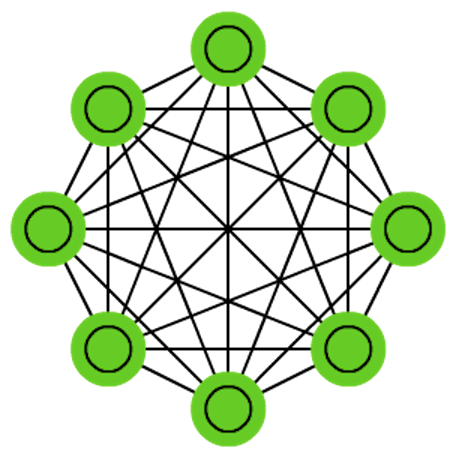
\includegraphics[scale=0.2]{img/agreen.png}
	\end{wrapfigure}
	\begin{alertblock}{Actor}
	Main \textsc{NN} which infers the action for a given state ($s_t\,\rightarrow\, a$)
	\end{alertblock}
	\vfill
	\begin{wrapfigure}{R}{0.3\textwidth}
		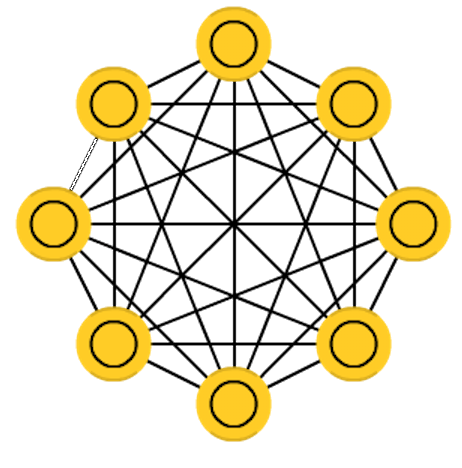
\includegraphics[scale=0.2]{img/ayellow.png}
	\end{wrapfigure}
	\begin{alertblock}{Critic}
	Secondary \textsc{NN} used only for training, evaluates the \textsc{actor} output returning the \textit{averaged} value of state-action pair. $s_t, a_t\,\rightarrow\, Q(s, a)$
	\end{alertblock}
\end{frame}

\begin{frame}{Advantage function for incremental learning}
	The \textsc{advantage} technique is used to give a  evaluation of the last action (reward) \textit{compared} to the average of other actions - so far performed - in a given state.
\pause

It answers the following question:	

	\centering
	\texttt{Is last action more rewarding than others in such scenario?}
\pause
	\begin{alertblock}{Yes}
		Action's likeliwood is encouraged i.e. actor gradients are pushed \textit{toward} this action.
	\end{alertblock}
	\begin{alertblock}{No}
		Action's likeliwood is discouraged i.e. actor gradients are pushed \textit{away} from this action. 
	\end{alertblock}
\end{frame}

\begin{frame}{Training}


\begin{figure}



\tikzset{every picture/.style={line width=0.75pt}} %set default line width to 0.75pt        

\begin{tikzpicture}[x=0.75pt,y=0.75pt,yscale=-1,xscale=1]
%uncomment if require: \path (0,300); %set diagram left start at 0, and has height of 300

%Image [id:dp9774282881643866] 
\draw (151,238) node  {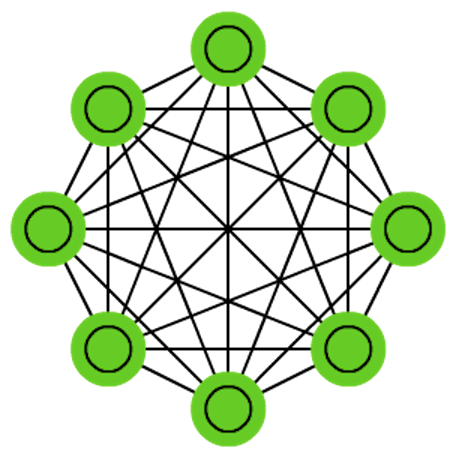
\includegraphics[width=52.5pt,height=52.5pt]{img/agreen.png}};
%Image [id:dp7868386159352238] 
\draw (223,158) node  {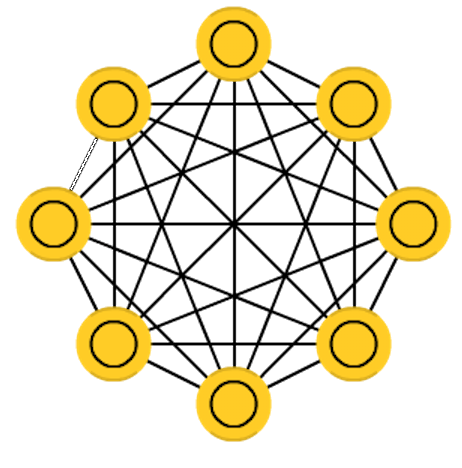
\includegraphics[width=52.5pt,height=52.5pt]{img/ayellow.png}};
%Shape: Rectangle [id:dp9886835947498787] 
\draw   (131,39) -- (252,39) -- (252,62.4) -- (131,62.4) -- cycle ;
%Straight Lines [id:da7272788353418506] 
\draw    (150,211.4) -- (150.99,66.4) ;
\draw [shift={(151,64.4)}, rotate = 450.39] [color={rgb, 255:red, 0; green, 0; blue, 0 }  ][line width=0.75]    (10.93,-3.29) .. controls (6.95,-1.4) and (3.31,-0.3) .. (0,0) .. controls (3.31,0.3) and (6.95,1.4) .. (10.93,3.29)   ;

%Straight Lines [id:da6350101234190333] 
\draw    (205,65.4) -- (205.97,132.4) ;
\draw [shift={(206,134.4)}, rotate = 269.17] [color={rgb, 255:red, 0; green, 0; blue, 0 }  ][line width=0.75]    (10.93,-3.29) .. controls (6.95,-1.4) and (3.31,-0.3) .. (0,0) .. controls (3.31,0.3) and (6.95,1.4) .. (10.93,3.29)   ;

%Straight Lines [id:da3606763379732807] 
\draw    (240,65.4) -- (240.97,132.4) ;
\draw [shift={(241,134.4)}, rotate = 269.17] [color={rgb, 255:red, 0; green, 0; blue, 0 }  ][line width=0.75]    (10.93,-3.29) .. controls (6.95,-1.4) and (3.31,-0.3) .. (0,0) .. controls (3.31,0.3) and (6.95,1.4) .. (10.93,3.29)   ;

%Shape: Diamond [id:dp8873126373500743] 
\draw   (224,222) -- (241,236.7) -- (224,251.4) -- (207,236.7) -- cycle ;
%Straight Lines [id:da11572660924853706] 
\draw    (223,191.4) -- (223.93,220) ;
\draw [shift={(224,222)}, rotate = 268.13] [color={rgb, 255:red, 0; green, 0; blue, 0 }  ][line width=0.75]    (10.93,-3.29) .. controls (6.95,-1.4) and (3.31,-0.3) .. (0,0) .. controls (3.31,0.3) and (6.95,1.4) .. (10.93,3.29)   ;

%Straight Lines [id:da7325386995610663] 
\draw    (103,239.4) -- (121,239.4) ;
\draw [shift={(123,239.4)}, rotate = 180] [color={rgb, 255:red, 0; green, 0; blue, 0 }  ][line width=0.75]    (10.93,-3.29) .. controls (6.95,-1.4) and (3.31,-0.3) .. (0,0) .. controls (3.31,0.3) and (6.95,1.4) .. (10.93,3.29)   ;

%Straight Lines [id:da481879043441071] 
\draw    (181,237.4) -- (207,236.7) ;


%Striped Right Arrow [id:dp2513873251906914] 
\draw   (280.25,138) -- (290.4,138) -- (290.4,128) -- (302,148) -- (290.4,168) -- (290.4,158) -- (280.25,158) -- cycle ;\draw   (273,138) -- (274.45,138) -- (274.45,158) -- (273,158) -- cycle ;\draw   (275.9,138) -- (278.8,138) -- (278.8,158) -- (275.9,158) -- cycle ;
%Image [id:dp9205816783587423] 
\draw (358,240) node  {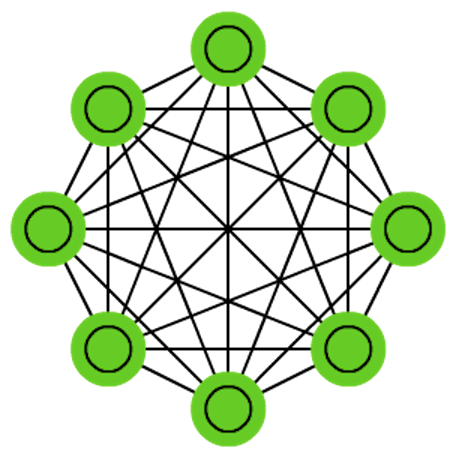
\includegraphics[width=52.5pt,height=52.5pt]{img/agreen.png}};
%Image [id:dp9906767747368865] 
\draw (430,160) node  {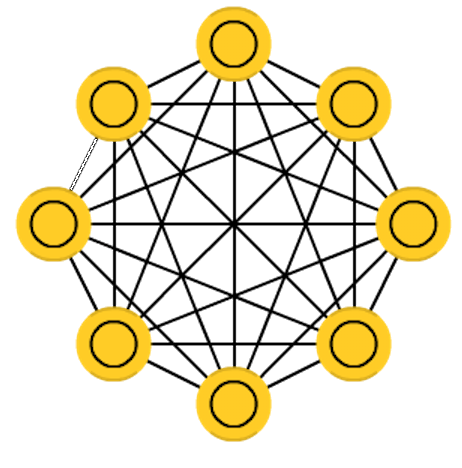
\includegraphics[width=52.5pt,height=52.5pt]{img/ayellow.png}};
%Shape: Rectangle [id:dp23908743254468723] 
\draw   (338,41) -- (459,41) -- (459,64.4) -- (338,64.4) -- cycle ;
%Straight Lines [id:da6388096580713554] 
\draw    (357,213.4) -- (357.99,68.4) ;
\draw [shift={(358,66.4)}, rotate = 450.39] [color={rgb, 255:red, 0; green, 0; blue, 0 }  ][line width=0.75]    (10.93,-3.29) .. controls (6.95,-1.4) and (3.31,-0.3) .. (0,0) .. controls (3.31,0.3) and (6.95,1.4) .. (10.93,3.29)   ;

%Straight Lines [id:da6482373157340046] 
\draw    (412,67.4) -- (412.97,134.4) ;
\draw [shift={(413,136.4)}, rotate = 269.17] [color={rgb, 255:red, 0; green, 0; blue, 0 }  ][line width=0.75]    (10.93,-3.29) .. controls (6.95,-1.4) and (3.31,-0.3) .. (0,0) .. controls (3.31,0.3) and (6.95,1.4) .. (10.93,3.29)   ;

%Straight Lines [id:da19125512768569786] 
\draw    (447,67.4) -- (447.97,134.4) ;
\draw [shift={(448,136.4)}, rotate = 269.17] [color={rgb, 255:red, 0; green, 0; blue, 0 }  ][line width=0.75]    (10.93,-3.29) .. controls (6.95,-1.4) and (3.31,-0.3) .. (0,0) .. controls (3.31,0.3) and (6.95,1.4) .. (10.93,3.29)   ;

%Shape: Diamond [id:dp31462774955284367] 
\draw   (431,224) -- (448,238.7) -- (431,253.4) -- (414,238.7) -- cycle ;
%Straight Lines [id:da9532701000531545] 
\draw    (430,193.4) -- (430.93,222) ;
\draw [shift={(431,224)}, rotate = 268.13] [color={rgb, 255:red, 0; green, 0; blue, 0 }  ][line width=0.75]    (10.93,-3.29) .. controls (6.95,-1.4) and (3.31,-0.3) .. (0,0) .. controls (3.31,0.3) and (6.95,1.4) .. (10.93,3.29)   ;

%Straight Lines [id:da7485811706491907] 
\draw    (310,241.4) -- (328,241.4) ;
\draw [shift={(330,241.4)}, rotate = 180] [color={rgb, 255:red, 0; green, 0; blue, 0 }  ][line width=0.75]    (10.93,-3.29) .. controls (6.95,-1.4) and (3.31,-0.3) .. (0,0) .. controls (3.31,0.3) and (6.95,1.4) .. (10.93,3.29)   ;

%Straight Lines [id:da6078020699023656] 
\draw    (388,239.4) -- (414,238.7) ;


%Striped Right Arrow [id:dp06691278122418354] 
\draw   (481.25,140) -- (491.4,140) -- (491.4,130) -- (503,150) -- (491.4,170) -- (491.4,160) -- (481.25,160) -- cycle ;\draw   (474,140) -- (475.45,140) -- (475.45,160) -- (474,160) -- cycle ;\draw   (476.9,140) -- (479.8,140) -- (479.8,160) -- (476.9,160) -- cycle ;

% Text Node
\draw (95,234) node [scale=1.2]  {$s_{0}$};
% Text Node
\draw (142,99) node [scale=1.2]  {$a_{0}$};
% Text Node
\draw (187,50) node  [align=left] {Environment};
% Text Node
\draw (213,99) node   {$s_{1}$};
% Text Node
\draw (250,99) node   {$r_{1}$};
% Text Node
\draw (112,51) node [scale=1.44]  {$t_{0}$};
% Text Node
\draw (302,236) node [scale=1.2]  {$s_{1}$};
% Text Node
\draw (349,101) node [scale=1.2]  {$a_{1}$};
% Text Node
\draw (394,52) node  [align=left] {Environment};
% Text Node
\draw (420,101) node   {$s_{2}$};
% Text Node
\draw (457,101) node   {$r_{2}$};
% Text Node
\draw (319,53) node [scale=1.44]  {$t_{1}$};
% Text Node
\draw (223,235) node  [align=left] {T};
% Text Node
\draw (430,237) node  [align=left] {T};


\end{tikzpicture}

\caption{Actor-Critic interactions in an iterative training}
\end{figure}
\end{frame}

\begin{frame}{Actor training}
	\begin{columns}[c]
		\begin{column}{0.5\textwidth}
			\begin{figure}
		



\tikzset{every picture/.style={line width=0.75pt}} %set default line width to 0.75pt        

\begin{tikzpicture}[x=0.75pt,y=0.75pt,yscale=-1,xscale=1]
%uncomment if require: \path (0,300); %set diagram left start at 0, and has height of 300

%Straight Lines [id:da031635540005715224] 
\draw    (110,129.4) -- (172,130.37) ;
\draw [shift={(174,130.4)}, rotate = 180.9] [color={rgb, 255:red, 0; green, 0; blue, 0 }  ][line width=0.75]    (10.93,-3.29) .. controls (6.95,-1.4) and (3.31,-0.3) .. (0,0) .. controls (3.31,0.3) and (6.95,1.4) .. (10.93,3.29)   ;

%Shape: Circle [id:dp3973148310809742] 
\draw   (285.6,129.2) .. controls (285.6,121.36) and (291.96,115) .. (299.8,115) .. controls (307.64,115) and (314,121.36) .. (314,129.2) .. controls (314,137.04) and (307.64,143.4) .. (299.8,143.4) .. controls (291.96,143.4) and (285.6,137.04) .. (285.6,129.2) -- cycle ;
%Shape: Folded Corner [id:dp8803770343896558] 
\draw   (163.08,99.4) -- (139,99.4) -- (139,73) -- (171,73) -- (171,91.48) -- cycle -- (163.08,99.4) ; \draw   (171,91.48) -- (164.66,93.06) -- (163.08,99.4) ;
%Image [id:dp9774282881643866] 
\draw (210,208) node  {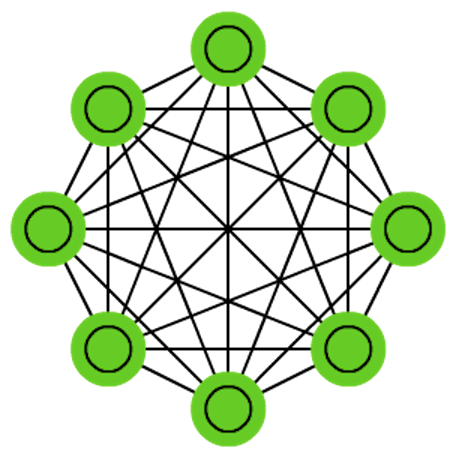
\includegraphics[width=52.5pt,height=52.5pt]{img/agreen.png}};
%Image [id:dp7868386159352238] 
\draw (211,130) node  {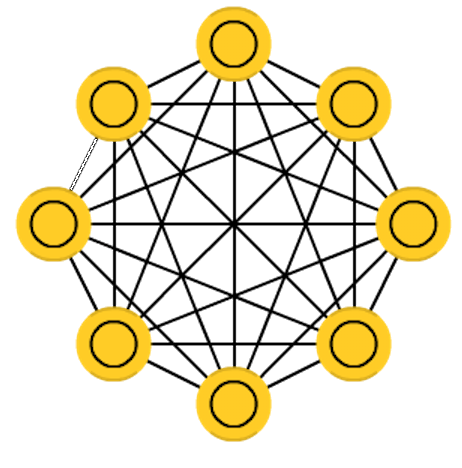
\includegraphics[width=52.5pt,height=52.5pt]{img/ayellow.png}};
%Straight Lines [id:da39368232370504685] 
\draw    (243,128.4) -- (283.6,129.16) ;
\draw [shift={(285.6,129.2)}, rotate = 181.08] [color={rgb, 255:red, 0; green, 0; blue, 0 }  ][line width=0.75]    (10.93,-3.29) .. controls (6.95,-1.4) and (3.31,-0.3) .. (0,0) .. controls (3.31,0.3) and (6.95,1.4) .. (10.93,3.29)   ;

%Shape: Folded Corner [id:dp7409201763808804] 
\draw   (162.08,186.4) -- (138,186.4) -- (138,160) -- (170,160) -- (170,178.48) -- cycle -- (162.08,186.4) ; \draw   (170,178.48) -- (163.66,180.06) -- (162.08,186.4) ;
%Curve Lines [id:da1487190598879865] 
\draw    (299.8,143.4) .. controls (305.94,204.78) and (306,208.33) .. (244.87,206.46) ;
\draw [shift={(243,206.4)}, rotate = 361.82] [color={rgb, 255:red, 0; green, 0; blue, 0 }  ][line width=0.75]    (10.93,-3.29) .. controls (6.95,-1.4) and (3.31,-0.3) .. (0,0) .. controls (3.31,0.3) and (6.95,1.4) .. (10.93,3.29)   ;

%Straight Lines [id:da7984862001037417] 
\draw    (116,54.4) -- (270,54.4) ;


%Curve Lines [id:da2563674197184984] 
\draw    (270,54.4) .. controls (312.36,51.44) and (298.44,79.54) .. (299.73,113.45) ;
\draw [shift={(299.8,115)}, rotate = 267.02] [color={rgb, 255:red, 0; green, 0; blue, 0 }  ][line width=0.75]    (10.93,-3.29) .. controls (6.95,-1.4) and (3.31,-0.3) .. (0,0) .. controls (3.31,0.3) and (6.95,1.4) .. (10.93,3.29)   ;

%Straight Lines [id:da9195593378431248] 
\draw    (171,91.48) -- (190,108.4) ;


%Straight Lines [id:da11232045611562991] 
\draw    (170,178.48) -- (189,195.4) ;


%Straight Lines [id:da09870551544175621] 
\draw    (125,130.4) -- (125,194.4) ;


%Curve Lines [id:da9974506407350556] 
\draw    (125,194.4) .. controls (124.02,212.13) and (133.7,210.46) .. (174.13,209.45) ;
\draw [shift={(176,209.4)}, rotate = 538.64] [color={rgb, 255:red, 0; green, 0; blue, 0 }  ][line width=0.75]    (10.93,-3.29) .. controls (6.95,-1.4) and (3.31,-0.3) .. (0,0) .. controls (3.31,0.3) and (6.95,1.4) .. (10.93,3.29)   ;

%Straight Lines [id:da6650284683134609] 
\draw    (115,245.4) -- (202,246.4) ;


%Curve Lines [id:da46792271663712803] 
\draw    (202,246.4) .. controls (191.5,244.49) and (207.44,251.7) .. (210.64,239.29) ;
\draw [shift={(211,237.4)}, rotate = 457.59] [color={rgb, 255:red, 0; green, 0; blue, 0 }  ][line width=0.75]    (10.93,-3.29) .. controls (6.95,-1.4) and (3.31,-0.3) .. (0,0) .. controls (3.31,0.3) and (6.95,1.4) .. (10.93,3.29)   ;


% Text Node
\draw (299,133) node  [align=left] {{\huge -}};
% Text Node
\draw (260,117) node   {$v_{t}$};
% Text Node
\draw (118,37) node [scale=1.2]  {$r_{t}$};
% Text Node
\draw (118,117) node [scale=1.2]  {$s_{t}$};
% Text Node
\draw (324,167) node [scale=1]  {$adv_{t}$};
% Text Node
\draw (118,232) node [scale=1.2]  {$a_{t}$};
% Text Node
\draw (153,84) node  [align=left] {1};
% Text Node
\draw (152,171) node  [align=left] {2};


\end{tikzpicture}

		\end{figure}
		\end{column}
		\begin{column}{0.5\textwidth}
			\centering
			\begin{itemize}
				\item\alert{1} Critic returns the averaged value of the state.
				\item\alert{2} Actor is trained considering $s_t$, $a_t$ and $adv_t =r_t-v_t$ 
			\end{itemize}
		\end{column}
		
	\end{columns}

\end{frame}


\begin{frame}[allowframebreaks]{References}

  \bibliography{rl}
  \bibliographystyle{abbrv}

\end{frame}
\end{document}
